% !TeX spellcheck = en_US
\documentclass[12pt]{article}

\usepackage{times,fullpage,xspace,fancyhdr,url,color}
\usepackage[pdftex]{graphicx}
\usepackage[pdftex,
            colorlinks=true,
            urlcolor=black,
            linkcolor=black,
            citecolor=black,
            bookmarksopen=false,
            bookmarksnumbered=true,
            pdfstartview=FitH]{hyperref}

\pdfcompresslevel=9
\newcommand{\leaguename}{RoboCup Standard Platform League (NAO) }
\hypersetup{
 pdftitle={\leaguename Technical Challenges},
 pdfauthor={Technical Committee SPL},
}
\usepackage{microtype}
\usepackage[utf8]{inputenc}
\usepackage{amsmath}
\usepackage{xargs}
\usepackage[colorinlistoftodos,prependcaption,textsize=tiny]{todonotes}
\usepackage{siunitx}
\usepackage[capitalize,noabbrev]{cleveref}
\usepackage[official]{eurosym}
\usepackage[useregional]{datetime2}
\usepackage{subcaption}
\usepackage{enumitem}
\usepackage{xcolor}
\DTMlangsetup[en-GB]{ord=raise,monthyearsep={,\space}}

\newcommandx{\unsure}[2][1=]{\todo[linecolor=red,backgroundcolor=red!25,bordercolor=red,#1]{#2}}
\newcommandx{\change}[2][1=]{\todo[linecolor=blue,backgroundcolor=blue!25,bordercolor=blue,#1]{#2}}
\newcommandx{\info}[2][1=]{\todo[linecolor=green,backgroundcolor=green!25,bordercolor=green,#1]{#2}}
\newcommandx{\improvement}[2][1=]{\todo[linecolor=Plum,backgroundcolor=Plum!25,bordercolor=Plum,#1]{#2}}

% comment 'disable' in to disable all the todo notes :)
\usepackage
[
%disable
]{todonotes}

\usepackage[theorems]{tcolorbox}
\newtcbtheorem[number within=section]{hintbox}{}%
{colback=red!10,colframe=red!45!black,fonttitle=\bfseries}{th}

% !TeX root = ../SPL-Rules.tex
% !TeX spellcheck = en_US
\newcommand{\TotalWidth}{7.4}
\newcommand{\TotalLength}{10.4}
\newcommand{\GoalScoredDelay}{15}
\newcommand{\KickOffAutoTime}{45}
\newcommand{\KickOffBallFreeTime}{10}
\newcommand{\FreeKickTime}{30}
\newcommand{\FreeKickRadius}{0.75}
\newcommand{\VisualSignalTime}{2}
\newcommand{\ReadyDelayTimeChampion}{45}
\newcommand{\ReadyDelayTimeChallenge}{40}
\newcommand{\PlayingDelayTime}{15}
\newcommand{\PenaltyKickTime}{30}
\newcommand{\PenaltyKickSetupTime}{30}
\newcommand{\PenaltyShootoutKickTime}{30}
\newcommand{\StandardPenaltyTime}{45}
\newcommand{\StandardPenaltyIncrease}{10}
\newcommand{\NovelContributionTime}{3 years\xspace}
\newcommand{\GameStuckTime}{30}
\newcommand{\TeamMessageSize}{128}
\newcommand{\TeamMessageLimit}{1200} % Limit of number of packets available to one team during a game with two halves of 10 minutes.
\newcommand{\TeamMessageLimitMinute}{60} % Limit for the average number of packets available to one team during a minute of gameplay.
\newcommand{\MaxJerseyNumber}{20} % the highest allowed jersey number to wear by robot players

% !TeX root = ../SPL-Rules.tex
% !TeX spellcheck = en_US
\newcommand{\LastRCYear}{2022\xspace}
\newcommand{\RCYear}{2023\xspace}
\newcommand{\JerseyApproveSubmissionDate}{2023-05-01}
\newcommand{\CodeReleaseAnnouncementDate}{2023-10-15}


\sloppy
\newcommand{\ie}{\mbox{i.\,e.}\xspace}
\newcommand{\eg}{\mbox{e.\,g.}\xspace}
%\newcommand{\cf}{\mbox{cf.}\xspace}
\newcommand{\cf}{see\xspace}
% \newcommand{\comment}[1]{\marginpar{\pdfannot width 4in height .5in depth 8pt {/Subtype /Text /Contents (#1)}}}
\newcommand{\inparagraph}[1]{\paragraph{#1\hspace{-1em} }}


% some colors
\definecolor{orange}{rgb}{1,0.5,0}
\definecolor{red}{rgb}{1,0,0}
\definecolor{green}{rgb}{0,1,0}


\title{\leaguename\\Technical Challenges}
\author{RoboCup Technical Committee}
\date{(\RCYear technical challenges, as of \today)}

\setlength{\parindent}{0pt}
\setlength{\parskip}{12pt plus 6pt minus 3 pt}
\setcounter{tocdepth}{1}
\widowpenalty=10000
\clubpenalty=10000

\pagestyle{fancy}
\lhead{}
\chead{}
\rhead{}
\lfoot{}
\cfoot{}
\rfoot{}

\renewcommand{\headrulewidth}{0.4pt}
\renewcommand{\footrulewidth}{0.4pt}

% needed to align an image and text correctly side by side
\newcommand{\imagebox}[1]{\raisebox{2ex}{\raisebox{-\height}{#1}}}

\begin{document}

\maketitle

\begin{center}
Questions or comments on the technical challenge rules should be submitted via \url{https://github.com/RoboCup-SPL/Rules/issues}, to the \texttt{\#rule-book} channel on the SPL Discord server, or by mail to \url{rc-spl-tc@lists.robocup.org}.
\end{center}

\newpage

\tableofcontents
\setcounter{tocdepth}{3}

\thispagestyle{fancy}

\clearpage

\cfoot{\thepage}
\setcounter{page}{1}

\section{Introduction}
At RoboCup \RCYear, the Standard Platform League will hold one technical challenge, which is described in this document.
RoboCup \RCYear awards a trophy for winning this challenge and the option for pre-qualification if a team is not pre-qualified by other means.

Technical challenges are used in the SPL to develop technical capabilities which will be used in upcoming RoboCups in the main competition. The purpose is to give teams time to develop solutions and exchange ideas before they will be introduced into the main competition. Challenges are designed to move the league in a direction of further improvement of soccer skills and towards the overall goal of 2050. Each team is strongly encouraged to participate in these challenges to contribute to the league's advancement.

\subsection{Code Publication}
Every team participating in a challenge must publish the corresponding code used in that competition according to Appendix A.7 of the SPL rule book, unless a specific challenge states otherwise.


% !TeX root = ../SPL-Challenges.tex
% !TeX spellcheck = en_US
\section{Shared Autonomy Challenge}

This technical challenge will challenge participants to develop a mixed team that consists of one human-operated Nao robot and one fully autonomous Nao. This challenge will consist of matches of two vs two robots on the standard SPL field. The exact number of matches will be subject to the number of available fields and the main competition schedule, however, teams should expect to participate in at least three matches.

\subsection{Challenge Goal}

This challenge takes a step towards the goal of enabling robots to play on the same field as agents with human level intelligence. To level the playing field in terms of physical embodiment, all players will be Nao robots. However, each team will have one of their robots be remotely operated by a human to provide human-level intelligence for robot control. The other robot will be fully autonomous in accordance with the main SPL competition rules.

\subsection{Challenge Rules}

This section details the complete rules to determine play and the winner of each match within the shared autonomy challenge. If not otherwise stated, the Champions Cup rules will be in effect.

\subsubsection{Team Composition}
Each participating team will set up one fully autonomous robot and provide one other robot that is programmed so that it can be operated by a human operator with restricted direct observation of the field, and one team member as the human operator.

\subsubsection{Limitations for Human Operation}
\begin{itemize}
	\item Each participating team will select the operator for their human-operated NAO from their registered team members.
	%
	\item Participating teams will design the appropriate interface for receiving field information from and sending controls to their human-operated robot.
	%
	\item The human operator will sit with their back to the field but close enough to hear referee whistles. The intention is that the operator cannot directly perceive the field but must do so through the controlled robot’s sensors.
	%
	\item The human-operated robot will be penalized if the operator turns and looks at the field.
	%
	\item The human operator may not receive other forms of game perception beyond what the operated robot can stream to it. This limitation includes 1) the human operator watching the challenge live feed on YouTube and 2) other team members with a view of the field communicating game information. However, due to the difficulty of prevention, teams will not be penalized if third-party spectators are overheard remarking on the game and then the human operator bases decisions on those remarks.
	%
	\item Teams are free to determine the operator interface subject to (1) the operator may not look at the field, (2) no teammate is allowed to communicate game information to the operator. The intention is that the operator may only have game information streamed from the human-operated robot and game controller. The referee has the discretion to bar unanticipated modes of communication that go against the spirit of this intention. 
	%
	\item The human-operated robot is not permitted to score goals directly on offense and may not take the goalkeeper role on defense.
\end{itemize}

\subsubsection{Limitations for Autonomy in the Human-Operated Robot}

For the human-operated robot, teams are encouraged to automate parts of control that would be difficult for human control. For example, the human operator may provide walk velocity commands that the robot then implements with a walk engine, or the operator may request a kick, and a kick engine generates the kick on the robot. The human operator may also set higher-level controls, such as the desired location to walk to. However, in the spirit of a mixed human-robot team, the human-operated robot must implement some form of a command from the human operator. That is, it is not permissible to participate in the challenge with two fully autonomous robots or to \textit{only} have the human operator augmenting the robot's perception and localization. 

\subsubsection{Number and duration of attempts}
Each match will give each team one attempt to play offense while the other team defends. An attempt will last 90 seconds or until the attacking team scores. The defending team is not permitted to score goals. If the defending team shoots the ball and it crosses the opponent’s goal line (so that in normal games, a goal would be scored), then a goal kick will be awarded to the attacking team. Effectively, we will treat the entire end line of the attacking team's side of the field as an out-of-bounds line. It is illegal to score directly off of kick off. Matches end in wins, losses, or draws depending on points scored, as described next. 

\subsubsection{Scoring matches}
Points will be awarded during matches on the basis of scoring goals and team coordination. To emphasize scoring on attempts, the attacking team receives two points for each successful goal scored. Teams may also receive additional points for passing where a qualifying pass consists of one robot on a team kicking the ball a distance of more than one (1) meter and then the teammate of the kicking robot making contact with the ball before a robot on the other team kicks or dribbles the ball. Here, a kick (or dribble) is taken to be any contact between a robot's foot while lifted off the ground with the ball. The intention is that incidental contact from the opponent does not disqualify a pass but that intentional contact does. For each qualifying pass, a team receives an additional point. The defending team may also score points via passes. Matches will be decided based on points and not on goals scored.

\subsubsection{Attempt Set-up}
All robots will be manually placed in their \textit{set} location by their team in order to speed up the time between attempts.  Attacking robots will be placed on one side of the field and the defending robots will be on the other side. The attacking team will try to score on the side where the defense starts. For defense, one robot will be designated as the goalkeeper and one as a field player. The goalkeeper must be the autonomous robot. The human-operated field player must be within the penalty area line to start.


\subsubsection{GameController and Penalties}
All robots have to communicate with the GameController. All rules from normal gameplay in the Champions Cup (including penalties) still apply unless explicitly changed here. The game controller operator will communicate the attempt time verbally at 30-second intervals to human operators.

\subsubsection{Network Conditions}
No guarantees are made about the conditions of the wireless network at the competition venue. No limits are placed on communication between the robot and the operator, however, attempts to jam the other team should not be taken. 

\subsubsection{Overall Challenge Scoring}
All participating teams will complete at least three matches and additional matches may be held as the main competition schedule allows. For purposes of deciding an overall challenge winner, the ranking will be based on the following in this order:
\begin{enumerate}
	\item Overall matches won.
	\item Highest score.
	\item Total successful passes.
	\item Goals scored.
\end{enumerate}
If a tie remains after all of these metrics are considered, then the winner will be determined by additional matches between the teams tied for top rank. The TC will determine a method for selecting opponents such that teams are appropriately matched in terms of strength.

\subsubsection{Code Release and Research Dissemination}
To foster the sharing of novel research and enable future development, all participating teams must:
\begin{enumerate}
	\item Prior to the first day of the challenge, submit up to two (2) .pdf slides presenting the team's approach to the competition. At a minimum, the slides should describe 1) the interface for the human operator, 2) the type of command the operator provides to the robot, and 3) the strategy for coordinating the human-operated and autonomous robot. To protect innovation during the competition, these slides will not be shared until after the first day of the challenge.
	\item  Release the code they develop for the human-operated robot (both robot code and interface code).
\end{enumerate}

\subsection{Miscellaneous Notes}

\begin{itemize}
\item Teams are given wide flexibility in interface implementation with the goal of inspiring innovation in how the challenge is addressed. For instance, a team could stream images from the human-operated robot but may face low bandwidth at the venue  (Note, the rules do not specify that any special effort will be made to provide stronger bandwidth for the challenge). Due to bandwidth constraints, teams may prefer to process images on board robot and send high level state info back to operator. However, this forces the operator to work with the robots imprecise state estimation. The choice is left as a research challenge for teams. 
\item Similarly, no specification is given on what control interface can be presented to the human operator. Teams may choose to directly command walk directions and kicks or to use a mixed autonomy mode where the operator gives high level directives that the human-operated robot implements. The only limitation is that the input from the operator must be some sort of command, i.e., it is not sufficient to only augment the robot's perception or localization.
\item Finally, the hardware of the interface (e.g., keyboard, joystick, virtual reality headset) is left up to the discretion of teams.
\item The defending team is not permitted to score because doing so may be too easy to counterattack with long kicks due to the field size and the limited size of teams.
\item Total expected time per match: 5 minutes (3 minutes playing and 2 minutes set up). 
\end{itemize}



% !TeX root = ../SPL-Challenges.tex
% !TeX spellcheck = en_US

\section{Leaderboard Challenges}
Starting in 2025, several leaderboards will be introduced to track and compare team performances across key skills
over multiple years. These leaderboards aim to motivate teams to improve in specific areas deemed valuable by the
league and to compile a record of the top-performing components and skills. By highlighting these individual skills,
the league encourages focused development in areas that contribute to overall team performance, and creates a showcase
of the best technical abilities in the league.

\subsection{Challenge Rules}
Each year, teams can choose to make an attempt at specific leaderboard challenges. The Technical Committee and Organizing
Committee will coordinate dedicated time slots at RoboCup for teams to complete their leaderboard attempts.
Metrics from each attempt will be recorded and added to the appropriate leaderboard. Each leaderboard will be based
on unique metrics and procedures, detailed below. Teams must indicate their intention for a leaderboard attempt 2 weeks before
the first competition day.

\subsection{Fastest Walk Leaderboard}
This leaderboard will measure how fast a NAO will be able to navigate along a both a straight path and one with obstructions.

\subsubsection{Setup}
This leaderboard challenge will take place on one half of a standard SPL field, and requires 1 active robot and 4 inactive robots.
Inactive robots will act as obstacles for half of the attempt and will be placed as follows (illustrated in \cref{fig:walk_leaderboard}):
\begin{itemize}
    \item On the penalty mark
    \item On both corners of the goal area that are not touching the field boundary
    \item On the corner of the goal area closest to the competing robot
\end{itemize}

The competing robot will be placed on the touchline, in line with the penalty mark.
The end goal is the touchline on the other side of the field.

\begin{figure}[t]
    \centerline{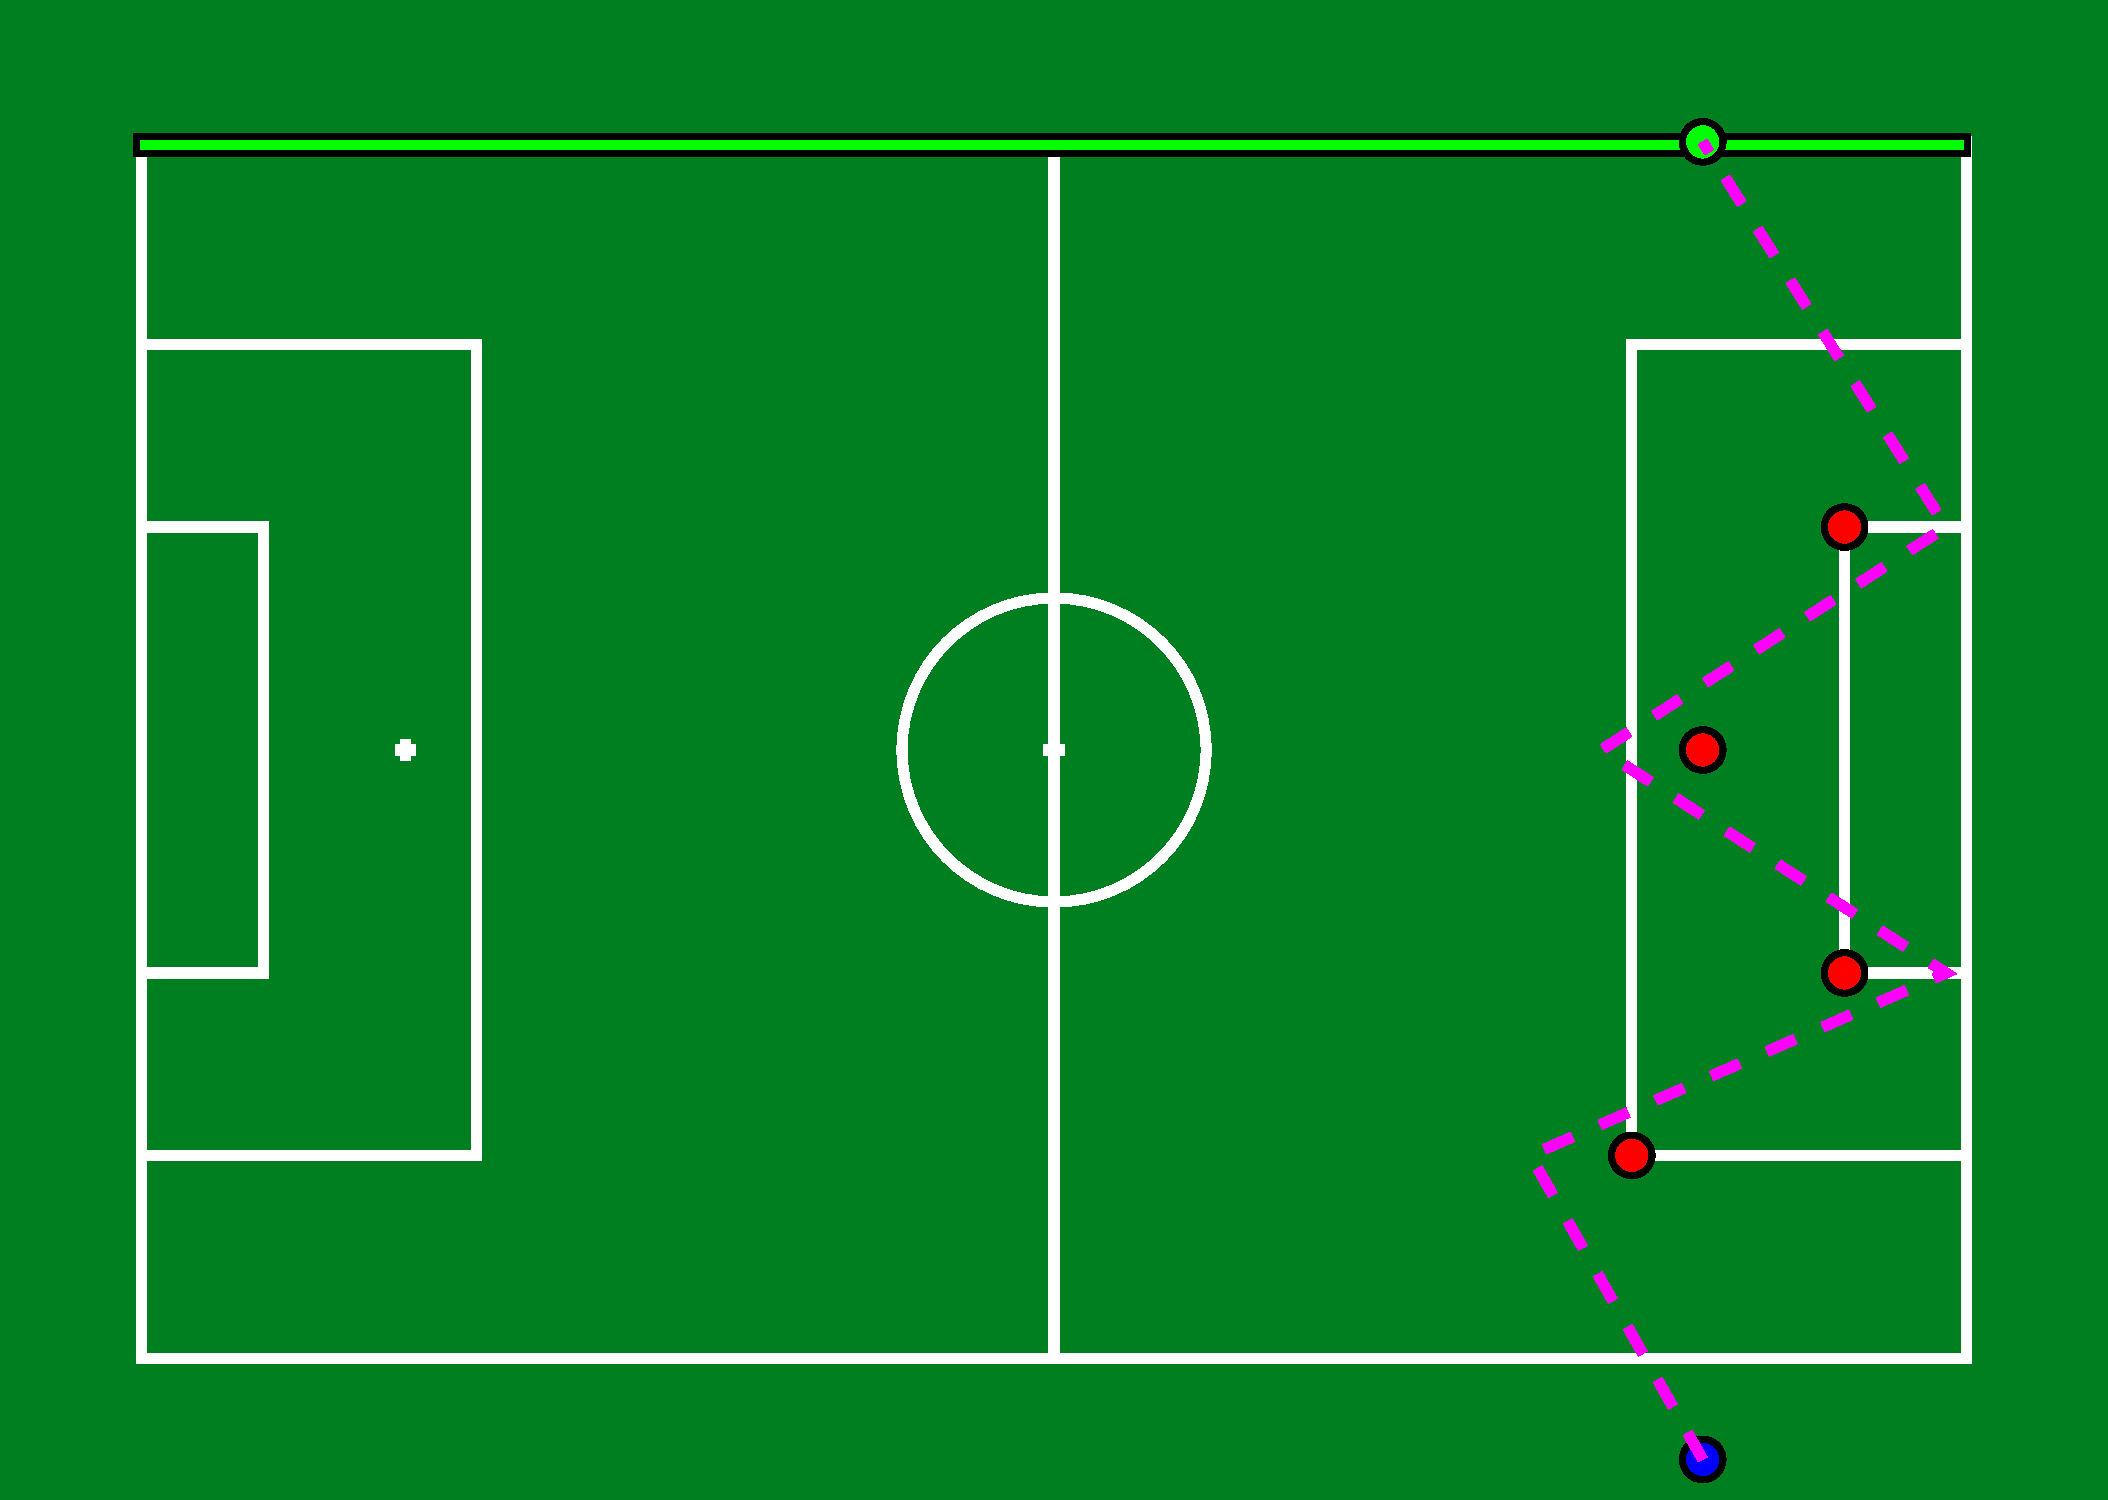
\includegraphics[width=\columnwidth]{figs/walk_leaderboard.pdf}}
    \caption{Fastest Walk Leaderboard: Robot completing the attempt is shown in blue, target is shown in green, obstacles are shown in red. An example path is shown in magenta}
    \label{fig:walk_leaderboard}
\end{figure}

\subsubsection{Challenge Execution}
Two types of runs will be completed, with three attempts per run allowed.

One run will be with the obstacles in place, where the active robot will need walk from it's
starting position to the target touchline, while weaving around the obstacle robots. (see \cref{fig:walk_leaderboard} for an example)

The other run will be with no obstacles, where the active robot will just need to walk 
to the target touchline.

Participating teams can choose which order they wish to complete these runs. Code changes are not allowed during a run,
but are allowed between runs.

Participating teams must start the robot behaviour of their competing robot via a single chest button
press (this mimics the chest button behaviour of switching between playing and penalized state).
The participating robot must navigate autonomously and cannot be remote controlled during the challenge

\subsubsection{Scoring}
Time starts from when the chest button is pressed, to when to robot entirely crosses the target touchline.

Teams will take 3 attempts at navigating both runs, with the sum of the lowest time for each
run being recorded in the leaderboard. Times will be rounded to the nearest second.

\subsection{Best Kick Leaderboard}
This leaderboard will measure how far and how accurate a NAO will be able to kick a standard
SPL soccer ball.

\subsubsection{Setup}
This leaderboard challenge will take place on a standard SPL field, and requires 1 active robot and 1 ball.
The ball will be placed on the centre of the edge of the goal area, in line with the penalty mark.
The competing robot will be placed in the centre of the goaline facing the ball
\begin{figure}[t]
    \centerline{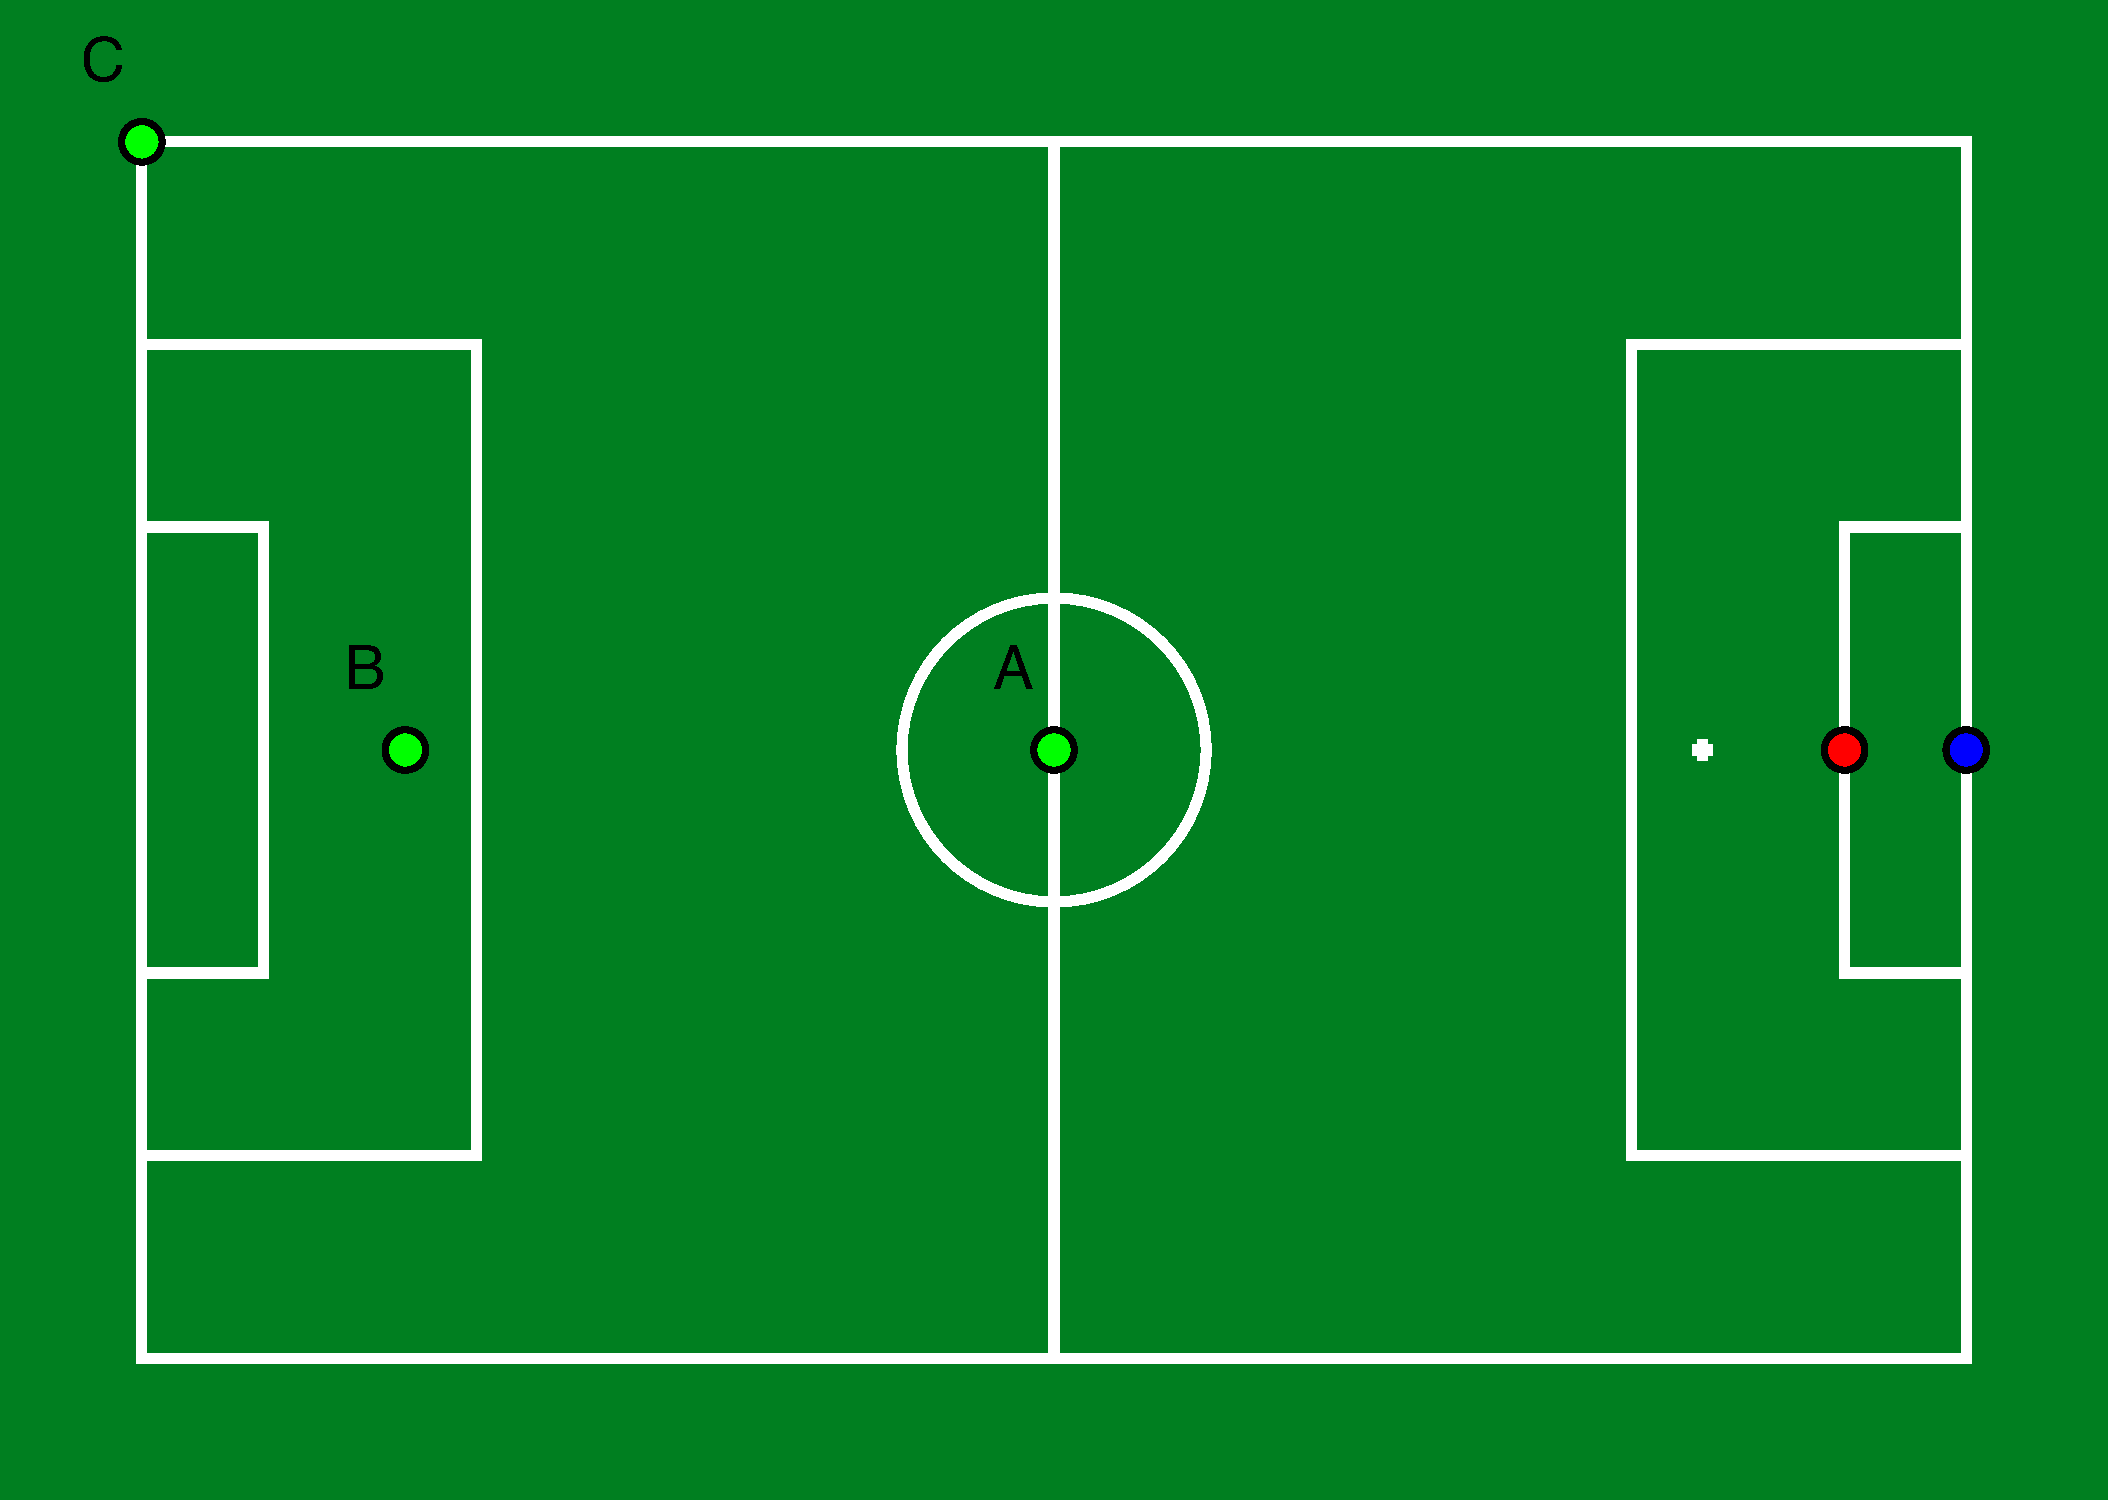
\includegraphics[width=\columnwidth]{figs/kick_leaderboard.pdf}}
    \caption{Best Kick Leaderboard: Robot completing the attempt is shown in blue, targets are shown in green, ball placement is shown in red}
    \label{fig:kick_leaderboard}
\end{figure}
\subsubsection{Challenge Execution}
Teams will be given 3 attempts at kicking to each of the 3 target postitions (illustrated in \cref{fig:kick_leaderboard}):
\begin{itemize}
    \item The centre mark in the centre circle
    \item The penalty mark on the opposite side of the field
    \item A corner on the opposite side of the field
\end{itemize}
In each attempt, participating teams must start the robot behaviour of their competing robot via a single chest button
press. The robot then has \qty{\PenaltyShootoutKickTime}{\second} to kick the ball towards the current target.
The competing robot must not touch the ball a second time after the ball has clearly moved,
otherwise the attempt ends immediately without scoring.
Once the ball has come to a complete stop, the distance from the ball to the target is measured.

Code changes are only allowed when changing targets.
\subsubsection{Scoring}
The sum of the smallest distance from each target will be recorded in the leaderboard.
Distances are rounded to the closest centimetre.

\subsection{Most Passes Leaderboard}
This leaderboard measures the highest number of successful passes a team can
complete in a given timeframe, emphasizing passing accuracy, speed, and coordination.

\subsubsection{Setup}
This leaderboard challenge will take place on a standard SPL field and requires 2 competing robots
and 1 standard SPL soccer ball.

Competing robots will be placed on the touchlines on opposite sides of the same half of the field,
in line with the penalty mark. The ball will be placed on the corner of the penalty area.

\begin{figure}[t]
    \centerline{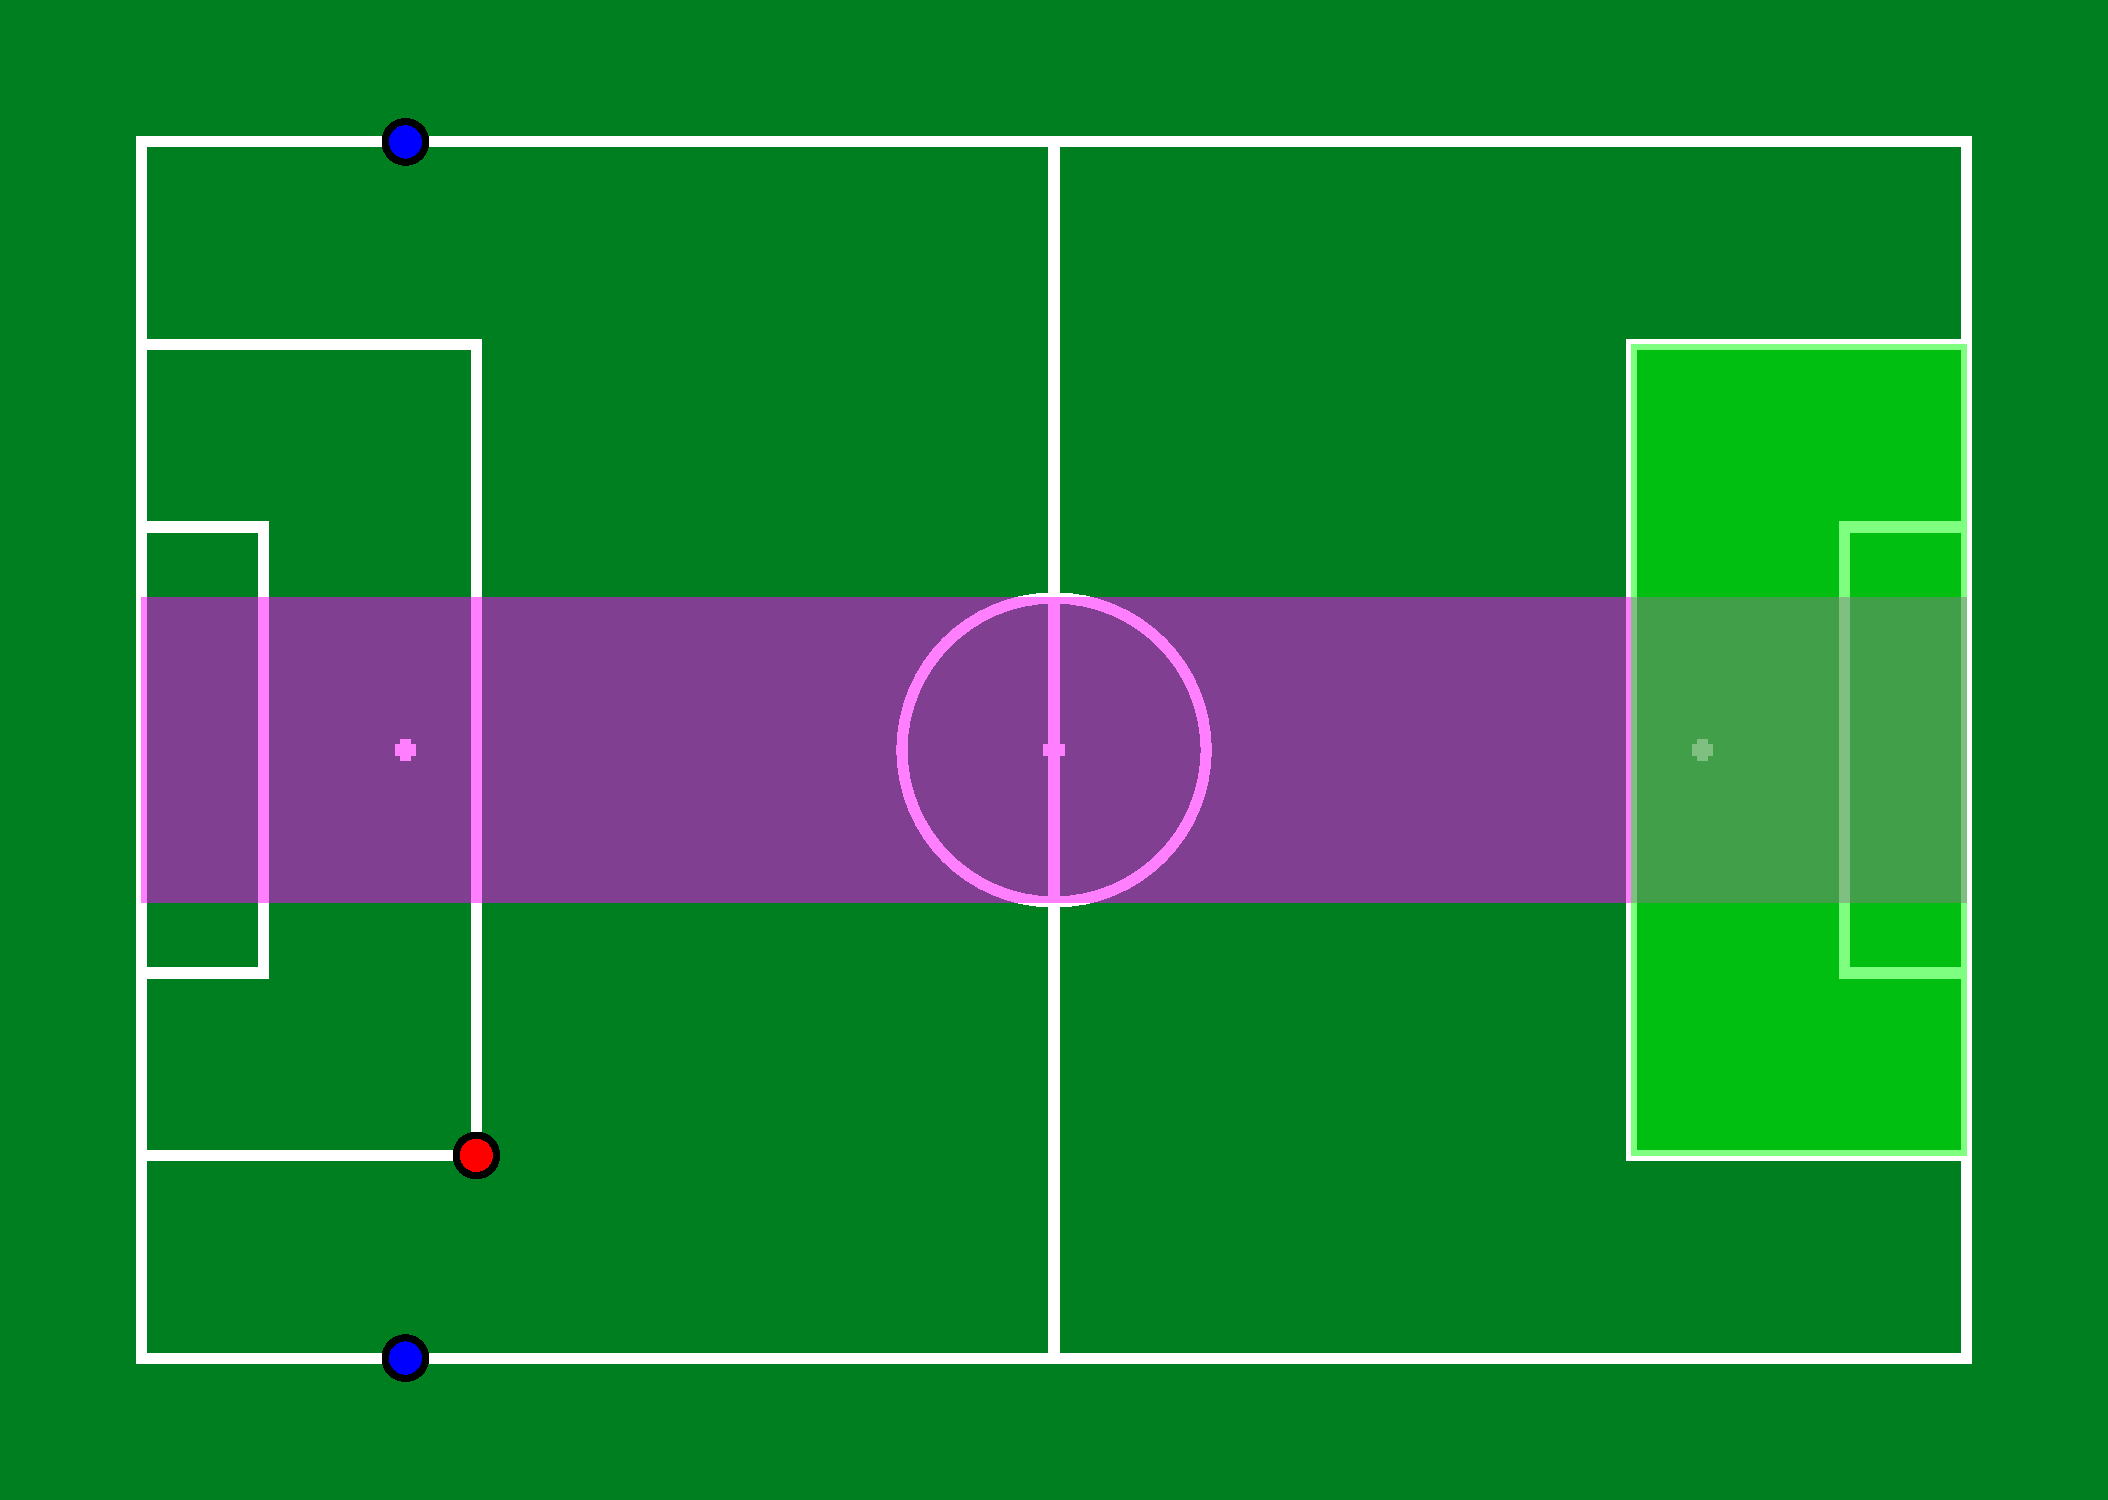
\includegraphics[width=\columnwidth]{figs/passing_leaderboard.pdf}}
    \caption{Passing Kick Leaderboard: Robots completing the attempt are shown in blue, target area is shown in green, exclusion area is shown in magents and ball placement is shown in red}
    \label{fig:passing_leaderboard}
\end{figure}
\subsubsection{Challenge Execution}
In each attempt, participating teams must start the robot behaviour of their competing robot via a single chest button
press. Teams will then have \qty{\MaxTimePassingLeaderboard}{\sec} to move the ball from the starting
position to the target area while completing as many passes as possible. The centre
1.5 metres of the field (Centre Cricle Diameter) is an exclusion zone, no robots are allowed within this area,
if a robot enters this area, or the ball comes to a complete stop
within this area, the run is ended immediately. If the ball is kicked off the field,
it is placed back on the touchline where it crossed. Each run is considered complete
once a robot has posession of the ball within the target area.

\subsubsection{Scoring}
1 point is awarded every time the ball crosses the exlusion zone, with an additional point
awarded if the ball touches the recieving robot before it stops rolling.

No points are counted if the time runs out before a robot has posession of the ball
within the target area, or if the run ends prematurely as per the above rules.

The highest score of the three runs will be recorded in the leaderboard.

\subsection{Ball Control Leaderboard}
This leaderboard will measure how well a NAO can keep control of a ball, while moving it
to a target.

\subsubsection{Setup}
This leaderboard challenge will take place on one half of a standard SPL field, and requires 1 active robot, 4 inactive robots and 1 SPL Soccer Ball.
Inactive robots will act as obstacles for the attempt and will be placed as follows (illustrated in \cref{fig:walk_leaderboard}):
\begin{itemize}
    \item On the penalty mark
    \item On both corners of the goal area that are not touching the field boundary
    \item On the corner of the goal area closest to the competing robot
\end{itemize}
The ball is placed on the touchline in line with the penalty mark, with the competing
robot placed around 50cm behind it.
The end goal is the touchline on the other side of the field.

\begin{figure}[t]
    \centerline{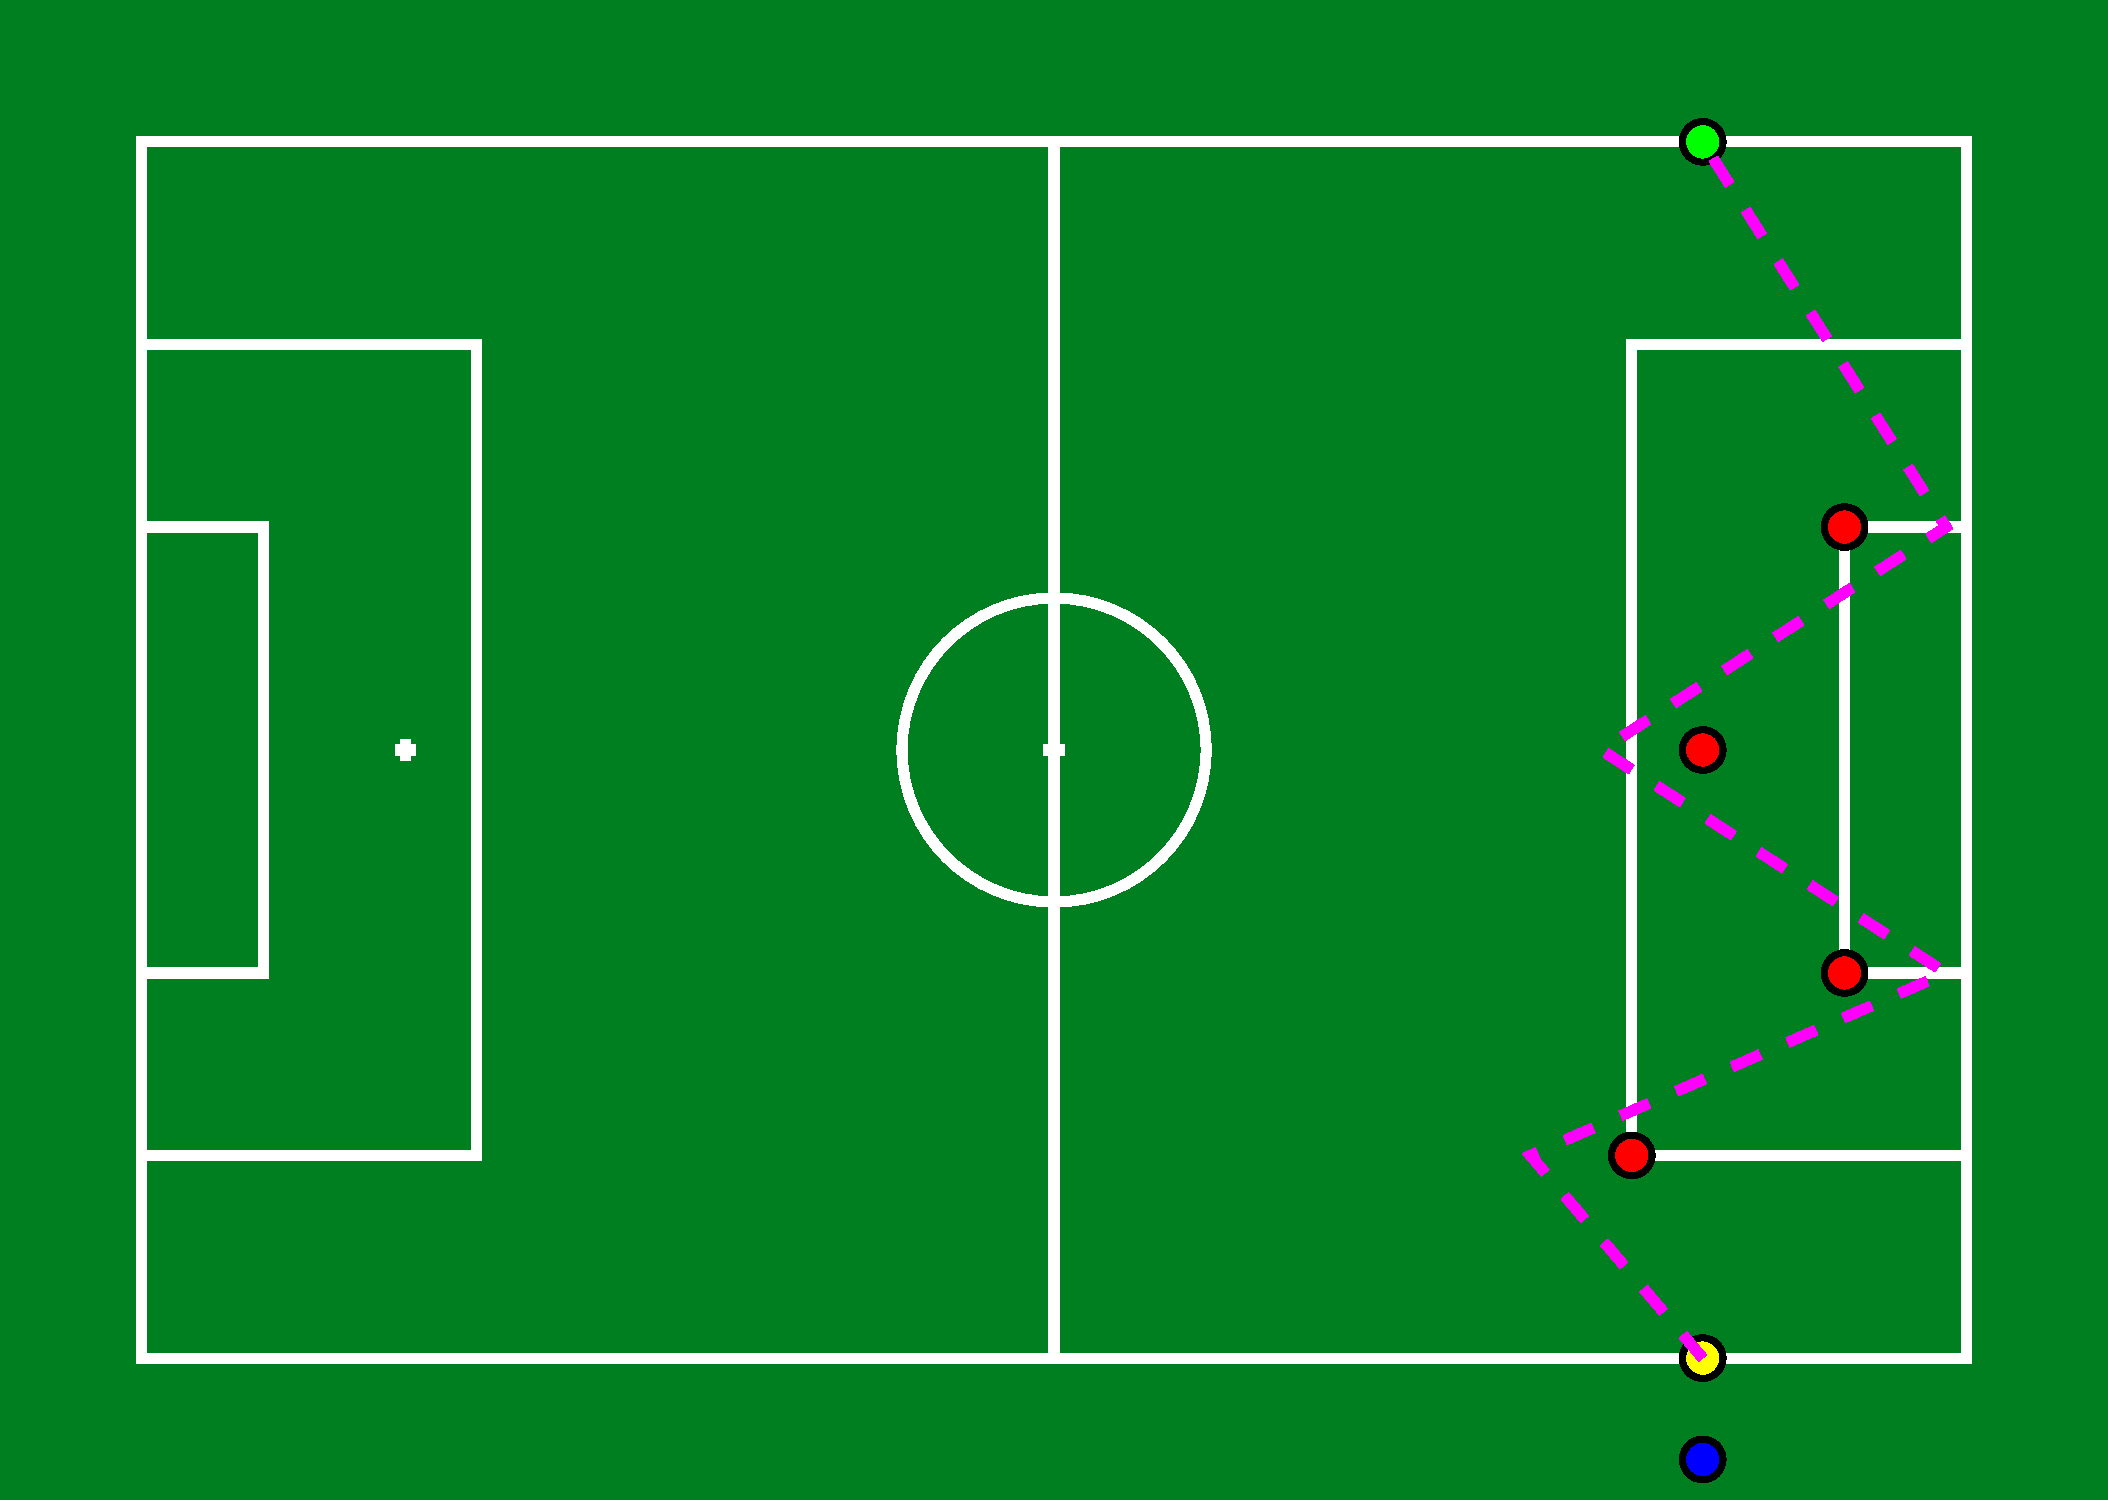
\includegraphics[width=\columnwidth]{figs/control_leaderboard.pdf}}
    \caption{Ball Control Leaderboard: Robot completing the attempt is shown in blue, target is shown in green, obstacles are shown in red and the ball is shown in yellow. An example path is shown in magenta}
    \label{fig:ball_control_leaderboard}
\end{figure}

\subsubsection{Challenge Execution}
In each attempt, participating teams must start the robot behaviour of their competing robot via a single chest button
press. Participating teams will be given 3 attempts to dribble the ball around the obstacles and across
the goal touchline in as fast a time as possible.

Anytime the ball moves more than 75cm away from the competing robot or the ball comes in contact with
and obstacle, a 30 second penalty we be added to the teams score.

\subsubsection{Scoring}
Time starts from when the chest button is pressed, to when to robot and ball entirely crosses the target touchline.

Teams will make 3 attempts, with the sum of all 3 attempts being recorded in the leaderboard.
Times will be rounded to the nearest second.

\subsection{Glicko Rating Leaderboard}
In addition to skill-specific leaderboards, the Glicko rating system will be updated to rank teams based on
performance consistency and competitiveness across various challenges and games.
The Glicko system will provide a dynamic rating that adjusts based on team performance
year-over-year, offering a comprehensive view of each team's standing in the league.

\subsubsection{Calculation}
...


\end{document}
